\section{Redes}

\subsection{Introducción a las redes}

Uno de los ejes fundamentales de este trabajo se basa en la utilización de redes neuronales para la detección y reconocimiento de patentes 
y sus correspondientes caracteres, entonces ¿Qué es una red neuronal?, a grandes rasgos una red neuronal en un algoritmo computacional que 
intenta imitar el cerebro humano, en otras palabras es un sistema de computación compuesto por un gran numero de elementos simples que se 
encuentran interconectados, los cuales procesan la información por medio de estados dinámicos, respondiendo a entradas externas
.[acá iría referencia]

Debido a la semenjanza que existe entre los algoritmos de deep learning y el cerebro humano, a la unidad fundamental de estos sistemas se la
 denomina neurona.
Cada neurona procesa la información de la capa de anterior y la entrega a la siguiente capa. Este proceso se puede entender como la sinapsis 
neuronal de los seres vivos.
La sinamsis es una suma poderada que puede ser expresada como $Y = W^T\dot X + b$ donde $W$ representa los pesos de la neurona, $b$ es un bias 
y $X$ es el vector de entrada.

Una capa es un arreglo en paralelo de neuronas, las capas se interconectan para crear redes más complejas capaces de realizar tareas más 
especificas [agregar figura de una red y sus partes].
Debido a que en esencia el proceso que realiza la neurona es una transformación lineal, al interconectar capas la resultante sigue siendo 
una transformación lineal. Este problema de linealidad se soluciona apilcando una función de activación luego de la transformación lineal, 
obteniendo $Y=f(W^T \dot X + b)$. [agregar grafico de funciones de activación].

Para realizar procesamiento de imagenes y extracción de características las redes mas utilizadas son las redes neuronales de combolución o 
CNN por sus siglas en inglés, ya que su diseño se basa en la estructura de la corteza visual animal, esta imitación se consigue utilizando 
convoluciones bidimensionales.
La convolución bidimensional es similar al caso conocido en 1D con algunas modificaciones, por ejemplo se habla de sistemas LSI (lineales de 
espacio invariante) en vez de LTI, para tenerla presente se procede a explicar la definición de convolución discreta en 2 dimensiones
Se define filtro, núcleo ó matriz de convolución a la respuesta de un sistema LSI discreto, el filtro es dimensión $2k x 2k$ donde $k$ es un 
valor establecido arbitrario (usualmente son matrices cuadradas de $3x3$ o $5x5$) que define cuantos valores habra de la muestra.
Se define a $h[n]$ como un filtro de dimension $2k x 2k$ e $I$ una imagen a escala de grises, donde cada punto de coordenadas $(i,j)$ es el 
resultado de la convolucion entre $h$ e $I$ dado por
\begin{equation}
    O(i,j)= \sum_{u=-k}^{k} \sum_{v=-k}^{k} h(u,v)I(i-u,j-v)
\end{equation}

Esta operacion consiste en filtrar una imagen de dimension $(2k+1)x(2k+1)$ en la imagen $I$ y para cada pixel centrado en dicha imagen, 
calculando la operacion de convolucion.
Es necesario definir algunos conceptos antes de continuar:
\begin{itemize}
    \item Paso $S_{w,h}$ distancia en pixeles que se da entre aplicacones sucesivas de la convolucion.
    \item Relleno cero $P_{w,h}$ numero de ceros que se deben añadir como borde al resultado de la convolucion.
\end{itemize}
(revisar si esto queda o no)

El ajustes de los filtros necesarios para extraer caracteristicas puede resultar un proceso largo y tedioso que no siempre conduce a los resultados que uno esperaria, por lo que se puede utilizar machine learning para obtener los valores de los filtros, para que se pueden extrar de manera satisfactoria las caracteristicas de las imagenes.

Para esta tarea, al colocar la neuronas en cuadriculas de $2k x 2k$, pueden usarse como filtros de convolucion para la extracion de caracteristicas y modificar sus valores durante la propagacion hacia atras (backpropagation, metodo de entrenamiento que sera explicado mas adelante)(ver tema de filtros en paralelo $F_d$ profunidad de filtro hiperparametro).

En este apartado se explicara como se compone una red CNN
\begin{itemize}
    \item Capa convolucional: capa principal de de las CNN, sus parametros son basicamente filtros entrenables de tamaño reducido, cada una de ellas produce un mapa de activacion bidimensional. Cada uno de estos filtros se activara segun la caracteristica que se busque.
    \item Capa de agrupacion: se coloca entre las capas de convolucion, toma los mapas de caracteristicas producidos por la capa de convolucion y los agrupa en una imagen. En esta capa se produce una reduccion de la dimesion, lo que reduce la complejidad para evitar el sobreajuste de los parametros.
    \item Capa de activacion: la unica funcion de esta capa es la de aumentar la no linealidad sin modificar los parametros, no son entrenables por lo que por ella solo se propagan los errores calculados.
    \item capa completamente conectada: tiene la estructura comun de una capa de nueronas pero con las particularidad que todas las neuronas de esta capa estan conectadas a todas las neuronas de la capa anterior.
    \item capa de perdida
\end{itemize}

Hablar de la arquitectura especifica de la yolov4?

HABLAR DE TIPOS DE NEURONAS CONVOLUCIONALES.

FALTA EXPLICAR EL ALGORITMO DE ENTRENAMIENTO MEDIANTE DATASETS Y BACKPROPAGATION.

Existen diversos tipos clasificación aunque la más utilizada es por el rol que la red puede desempeñar, existen redes reunorales convolucionales o CNN por sus siglas en inglés (comúnmente utilizadas para clasificación de imagenes),
redes neuronales recurrenter o RNN (utilizadas para predicción de texto de largo variable), entre otras. Otra clasificación que es posible utilizal es según la cantidad de capas que esta posea, existiendo 2 clasificaciones, simple las cuales no poseen capas ocultas y profundas las cuales si poseen capas ocultas.

A continuación se dará un breve resumen de como se crean estas capas de neuronas, para ello vamos explicar de manera sencilla y concisa como funciona una red neuronal:
\begin{itemize}
    \item Una capa recibe valores, llamados inputs,si se trata de la primera capa esos valores vendrán definidos por los datos de entrada, mientras que el resto de capas recibirán el resultado de la capa anterior.
    \item Luego se realiza una suma ponderada de todos los valores provenientes de la entrada, para ellos se necesita una matriz de pesos llamada W, la matriz tiene filas igual al numero de de capas anterior y columnas igual como neuronas tiene la capa actual.
    \item Al resultado de la suma ponderada se le sumará otro parámetro, conocido como bias o, simplemente, b. Cada neurona tiene su propio bias, por lo que las dimensiones del vector bias depende de la capa, por lo que será una columna y tantas filas como neuronas tiene esa capa.
    \item Luego se requiere de una función de activación, uno de los elementos mas importantes dentro de la red. Ya que hasta ahora solo tenemos una regresión lineal. Para evitar esto, al resultado de la suma anterior se le aplica una función, conocido como función de activación. El resultado de esta función será el resultado de la neurona.
\end{itemize}

Una vez que se realiza la suma ponderada, lo que tenemos es básicamente una transformación lineal, por lo que para evitar esto, se introduce una función que modifica estos datos, conocida como función de activación, que ademas de sacar linealidad a la red, le permite resolver problemas mas complejos, algunas de las mas usadas son la funcion escalon, la funcion sigmoide, la funcion rectificadora ReLU y la funcion tangete hiperbolica.[poner graficos]


vamos a hablar sobre redes neuronales basadas en imágenes (CNN) y sobre yolo v4.

\begin{figure}
    \centering
    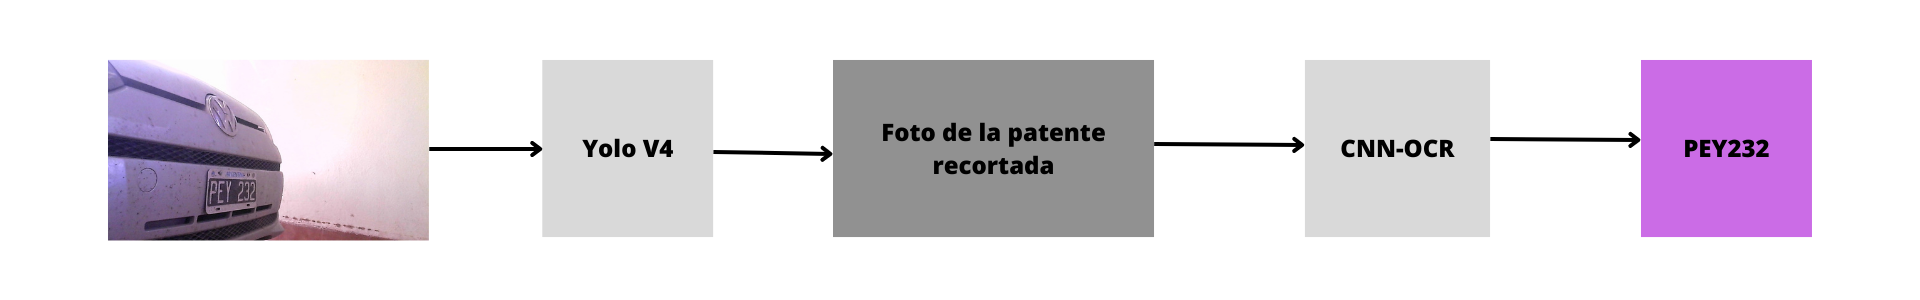
\includegraphics[width=\textwidth]{imgs/algoritmo-deteccion-patente.png}
    \caption{Algoritmo de OCR implementado.}
\end{figure}


\subsection{YoloV4}

Explicación YoloV4

\subsection{CNN-OCR}

Explicación de la CNN que reconoce caractere, porque se utilizo un CNN y no un LSTM (más habitual en tareas de predicción de texto)


\subsection{Nuestro algoritmo de detección}

Se pretende hablar sobre la implementación paso a paso del algortimo, uniendo los conceptos vistos hasta ahora, realizando una explicación breve de como se realiza la conversión de foto a texto.

\begin{figure}
    \centering
    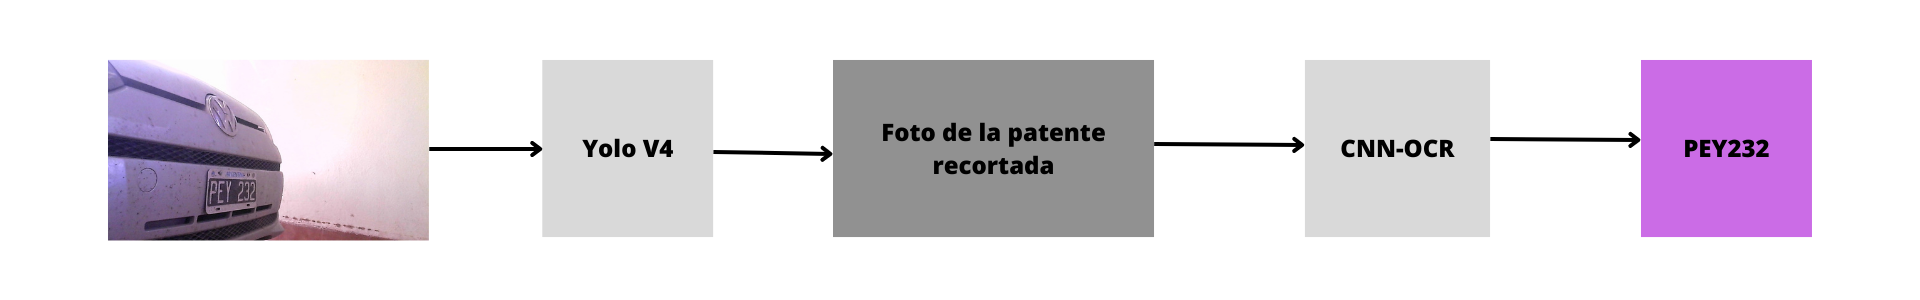
\includegraphics{imgs/algoritmo-deteccion-patente.png}
    \caption{Resumen gráfico del algoritmo paso a paso.}
\end{figure}